\chapter{EXPERIMENT AND RESULTS}
\thispagestyle{fancy}

    Based on the presented concepts thus far, our presented Adam-DQL algorithm relies on applying a faster gradient optimization technique to an already established Deep Q-Learning techniques made by Deepmind. Despite the wide range of possible applications (especially in modern games), as a proof of concept, this thesis narrowed down to a handful of illustrative environments that represents varied elements in modern video games. Adam-DQL agent is deployed, then tested on these environments, followed by a thorough analysis and insights about how the agent is performing on these environments.
    
    \section{Experimental Setup}
    In all experiments, the following definitions are used:
    \begin{itemize}
        \item \textit{Timesteps} is a unit used to indicate the simulation or game time. For every timestep, images/frames are fed into the neural network. This term can be used interchangeably with \textit{frames}.
        \item \textit{Episode} is an entire play of the game from the start until the game over signal, or often referred as terminal state. 1 episode could last for few hundred frames.
        \item \textit{Raw pixels} is the unprocessed raw values from a screen capture of a game.
        \item \textit{State} is a preprocessed image from the game, that is ready to be fed into the neural network. 
        \item \textit{Local Minima} indicates a point where the value of the error or loss function is smaller than all the neighboring points
        \item \textit{Global Minima} indicates a point where the value of the error or loss function is the smallest across all points.
        \item \textit{Regression} (programming terms) is a condition where a program becomes worse throughout updates.
        \item \textit{Annealing} means linearly reducing the value of a variable.
        \item \textit{Oscillates} is a condition where an AI agent stays on the same level of performance because of regression-improvement loop.
        \item \textit{Policy} indicates a function $\pi: S \to A$ that maps state into an action. 
    \end{itemize}
    
    In all experiments, the following setup was used:
    \begin{itemize}
        \item All of the environments used in this thesis are made on Python 2.7.3. All GUI elements are drawn on top of PyGame and Python-tk toolkit.
        \item Adam-DQL agent are built on top of Google's deep learning library, Tensorflow. Specifically, Tensorflow 1.7.0b.
        \item Adam-DQL agent are implemented as a Python class/module for future reuse and research purposes.
        \item Adam-DQL is trained using GPU-CUDA with the following specifications:
        \begin{table}[H]
            \centering
            
            \label{specs}
            \begin{tabular}{|l|l|l|}
            \hline
            \textbf{Server Name}     & \textbf{Desktop}    & \textbf{Laptop}     \\ \hline
            \textbf{OS}              & Ubuntu 18.04        & Ubuntu 16.04        \\ \cline{1-1}
            \textbf{Num. CPU's}      & 4                   & 8                   \\ \cline{1-1}
            \textbf{CPU Clock Freq.} & 3.1 GHz             & 2.8 GHz             \\ \cline{1-1}
            \textbf{Num. CPU Cores}  & 4                   & 8                   \\ \cline{1-1}
            \textbf{Ram Size}        & 8 GB                & 16GB                \\ \cline{1-1}
            \textbf{GPU 1 Type}      & Geforce GTX 750 Ti & Geforce GTX 1050 Ti \\ \cline{1-1}
            \textbf{GPU 1 mem. size} & 2 GB                & 4 GB                \\ \hline
            \end{tabular}
            \caption{Hardware Specifications}
        \end{table}
        \item The result points are taken every 10000 training episodes, unless stated otherwise (for comparison purposes).
        \item The training process ends at 500000 episodes unless the neural network doesn't grow any further before 500000 episodes.
        \item The value of the reward at every point is the average reward from 100 games played by the agent at that checkpoint.
        \item Since this is a reinforcement learning problem, the same datasets are used for training and validation.
    \end{itemize}
    \section{Architecture Analysis}
    
    Before Adam-DQL agent can be tested on our proposed environments, The software framework architecture needs to be finalized first. The chosen architecture is already shown in Chapter \ref{sec:4}, nevertheless, the reasoning behind that decision is still unclear. This section will go in depth on all the possible architecture and justify the decision on the last chapter. There's 3 possible software architecture for Adam-DQL, namely 1-block, 2-blocks and 3-blocks system.
    
    \subsection{1-block architecture}
         The 1-block architecture, as the name suggests, consist of only one software block. This means that the testing environment (the game) and the agent is merged into one program. The game will be modified heavily, and the agent will be integrated inside the game's code. This is the ideal scenario for practical usage of the AI, as this is the architecture that a normal game with AI will use in real life. However, this architecture is not suitable for testing and educational purposes, as the agent's code is made to work only with this specific environment. Changing environment (testing other game) means creating a new software from scratch. In layman terms, this architecture is the least general of all 3, while also being the cleanest and the fastest, because there's no inter-program communication involved.
         
        \begin{figure}[H]
            \centering
            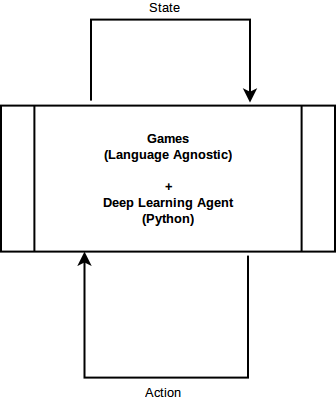
\includegraphics[scale=0.5]{images/framework1block.png}
            \caption{The 1-block architecture}
            \label{fig:1block}
        \end{figure}
 
    \subsection{2-blocks architecture}
        The 2-blocks architecture, consist of 2 software blocks, the environment (the game) and the agent. This means that the testing environment is separated from the agent, and only modified slightly to accommodate the requirements of the agent. The environment will send the raw pixels (image) to the agent, and agent will perform the preprocessing step, resulting in the actual state required by Adam-DQL algorithm. The agent will then perform Adam-DQL algorithm and send the best action back to the environment, and the environment will perform that action. This architecture will work generally for most games. However, some games are built like a "blackbox", and these modifications might not be possible. This architecture utilizes few inter-program communication, which might be a bit challenging to build. As this architecture seems to provide the balance between generality, ease of development and speed, this architecture is then \textbf{chosen for this thesis}.
        
           \begin{figure}[H]
            \centering
            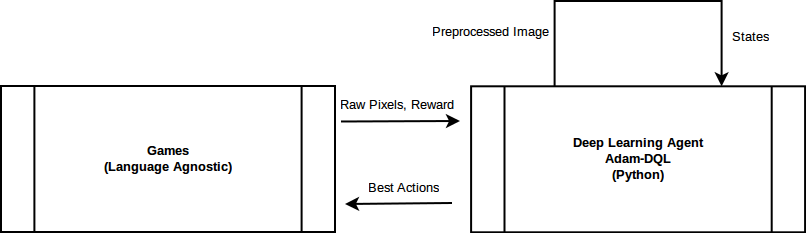
\includegraphics[scale=0.4]{images/framework2block.png}
            \caption{The 2-block architecture}
            \label{fig:2block}
        \end{figure}
 
    \subsection{3-blocks architecture}
        The 3-blocks architecture is the most complex architecture that Adam-DQL can use. This architecture utilizes some kind of middleware, the third program that translates the raw data from the game into the usable data (state) for the agent. The game only sends the memory buffer, and the middleware will read the memory buffer and translates it into preprocessed image (state) and reward. This data will be processed by the agent, to receive the best action for that state. Instead of sending the action directly into the game, this action will be sent into the middleware, and the middleware will simulate a keyboard/input that corresponds to that action. This way, there's almost no modification needed for the environment, thus resulting in the most general architecture. However, this architecture is the least trivial to implement, requiring low-level (memory level) knowledge for every game, and also the slowest. This architecture is what deepmind used in their publications, resulting in them being able to test on a huge set of games \cite{mnih2015humanlevel}.
           \begin{figure}[H]
            \centering
            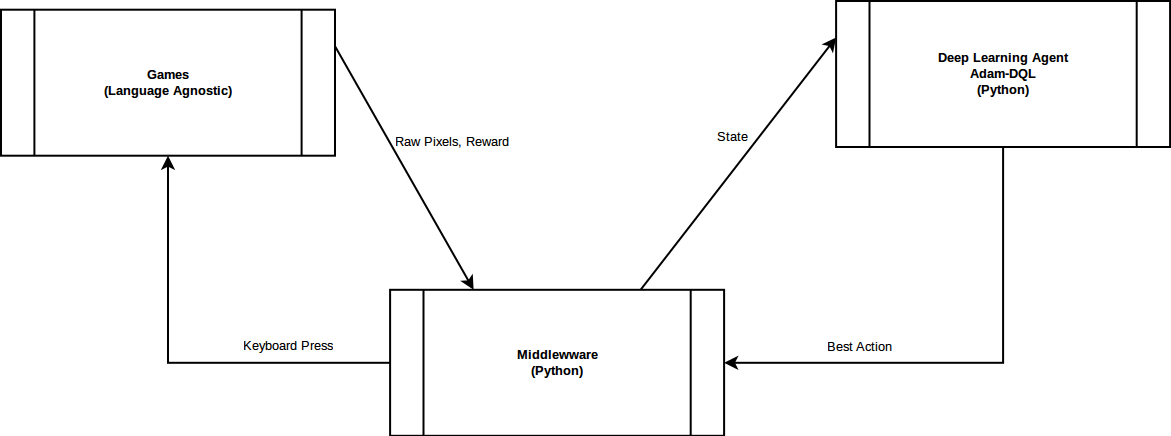
\includegraphics[scale=0.33]{images/framework3block.png}
            \caption{The 3-block architecture}
            \label{fig:3block}
        \end{figure}
        
    
 
        
  \section{Proposed Environments} \label{environment}
	
	Below are some game environments that will be used to test the learning capability of Adam-DQL. These game environments are specifically chosen to showcase Adam-DQL's ability to learn different type of games. The purpose of each chosen environment will be explained on the second part of this chapter. As explained in Section \ref{sec:4}, These information aren't given to the Adam-DQL agents instead are meant to give readers an idea about the testing environment (difficulties and types). The agents itself only receive raw pixels (as states) and rewards. 
	\subsection{Cartpole/Inverted Pendulum}
    	   
    Consider tasks in which an agent interacts with an environment,
    in this case a simplified inverted pendulum problem without friction, often referred as cartpole \cite{bartosutton}.  A pole is attached by an un-actuated joint to a cart, which moves along a frictionless track. Our main goal is to balance the pole by utilizing an applied force to both left and right ends of the cart.
    
    \begin{figure}[H]
        \centering
        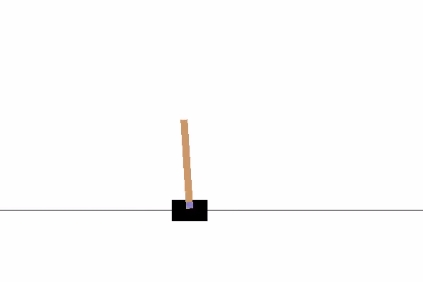
\includegraphics[scale=0.5]{images/cartpole.png}
        \caption{Image of the OpenAI Gym's Cartpole problem}
        \label{fig:51}
    \end{figure}
    
    The problem dynamics has the following equation, with $x$ being the horizontal position of the cart, and $\theta$ being the angle of the pole and the vertical axis:
    
        \begin{gather*}
                 x_{t+1}=x_t+\tau \dot{x_t}\\
            \dot{x}_{t+1}=\dot{x_t}+\tau \ddot{x_{t}}\\
            \ddot{x_t}=\frac{F+ml(\dot{\theta_t^2} sin(\theta_t) - \ddot{\theta_t}cos(\theta_t)}{m+M}\\
             \theta_{t+1}=\theta_t+\tau \dot{\theta_t}\\
            \dot{\theta}_{t+1}=\dot{\theta_t}+\tau \ddot{\theta_{t}}\\
            \ddot{\theta_t}=\frac{g sin(\theta_t) - cos(\theta_t)\frac{-F-\dot{\theta_t^2}sin(\theta_t) }{m+M}}{l(\frac{4}{3}-\frac{m cos(\theta_t)^2}{m+M})}\\
        \end{gather*}
       
       where $\tau = 0.02$(seconds/step), the length of the pole $l = 0.5(m)$, $F = \pm10$ is the magnitude of the force applied by our agent. The mass of the pole is $m = 0.1(kg)$, mass of the cart $m = 1.0(kg)$ and gravity $g = 9.8(ms^{−2} )$. It's important to note that equations above aren't differential equations, rather, a simplified algebraic equations representing the same problem.
       \begin{itemize}
        \item \textbf{Environment dynamics $s_t$} : $(x_t,\dot{x}_t,\theta_t,\dot{\theta}_t) \in S$, consisting of a state for the agent, following the dynamics presented above. The starting position is $s_0$ , a uniform randomized 4-D vector with boundaries for each variable of $[-0.05,0.05]$. The goal is to balance the pole for 195 timesteps in average. Mathematically balancing the pole means, keeping $||x_t|| \leq 2.4(m)$ or $||\theta_t||\leq\frac{24}{360}(rad)$.
        \item \textbf{A finite (2) set of actions A}, Apply force to the left $(a=-1 : F=-10(N))$ or apply force to the right $(a=1 : F=10(N))$.
        \item \textbf{A reward function} $r=R(s_t,a_t,s_{t+1})$, which is $r=1$ for every timestep in which the agent managed to prevent the game from ending.
    \end{itemize}
    \subsection{FlapPy Bird}
    
    Consider a tasks which an agent interacts with an environment, in this case a game where the agent controls a bird crossing a gap between pipes. This environment is heavily inspired by a popular mobile game \textit{Flappy Bird} by Dong Nguyen in May 2013. A bird can "\textit{flap}" to prevent falling due to gravity, or to prevent contact with the pipes. Our main goal is to control the bird (flapping) to make sure it crosses maximum number of gaps before falling or making contact with pipes.
    
     \begin{figure}[H]
        \centering
        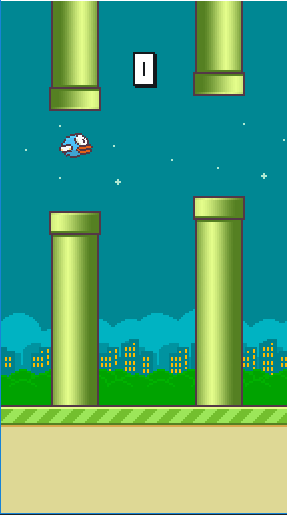
\includegraphics[scale=0.5]{images/flappy.png}
        \caption{Image of FlapPy Bird, reimplementation of Flappy Bird designed for Adam-DQL testing environments}
        \label{fig:52}
    \end{figure}
    
     \begin{itemize}
        \item \textbf{Environment dynamics $s_t$} : $(x_t,\dot{x}_t,\theta_t,\dot{\theta}_t) \in S$, consisting of a state for the agent, following the description presented above. The starting position is $s_0$, a 2D vector $x_0$ and $y_0$ representing the starting position of the bird. The goal is to use bird's flapping ability to cross the gap between pipes. The height of the pipes is uniformly distributed random variable between $[10,90]$. Gap width between upper and lower pipes is uniformly distributed random variable between $[20,60]$.
        \item \textbf{A finite (2) set of actions A}, Flap ($v_y+=9$(m/s)) or do nothing.
        \item \textbf{A reward function} $r=R(s_t,a_t,s_{t+1})$, which is $r=0.1$ for every timestep where the agent doesn't make contact or crosses the pipe. $r=1$ every time the agent crosses a pipe successfully, and $r=-1$ every time the agent makes contact with pipe or ground (thus ending the game/episode).
    \end{itemize}
    
    \subsection{Simplified Tetris}
    
    Consider a tasks which an agent interact with an environment, in this case a simplified version of a classic puzzle game, Tetris. Tetris is a tile-matching puzzle game that involves pieces called Tetriminos. Tetriminos are game pieces shaped like tetrominoes, geometric shapes composed of four square blocks each. A random sequence of Tetriminos fall down the playing field (a rectangular vertical shaft, called the "grid" or "matrix"). The objective of the game is to manipulate these Tetriminos, by moving each one sideways (if the player feels the need) and rotating it by 90 degree units, with the aim of creating a horizontal line of ten units without gaps. When such a line is created, it gets destroyed, and any block above the deleted line will fall. When a certain number of lines are cleared, the game enters a new level. As the game progresses, each level causes the Tetriminos to fall faster, and the game ends when the stack of Tetriminos reaches the top of the playing field and no new Tetriminos are able to enter.
    
       \begin{figure}[H]
        \centering
        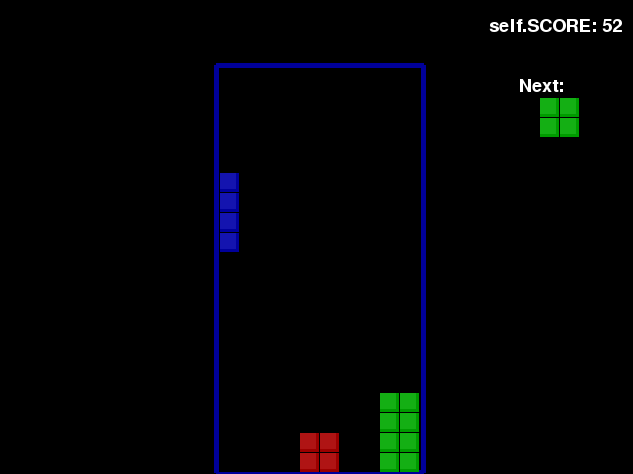
\includegraphics[scale=0.4]{images/tetromino.png}
        \caption{Image of Tetromino, reimplementation of Tetris designed for Adam-DQL testing environments}
        \label{fig:53}
    \end{figure}
      
     \begin{itemize}
        \item \textbf{Environment dynamics $s_t$} : $(b_t,b_{t+1},G_t) \in s$. $b_t$ represents the current falling block at time $t$, and $G_t$ represents the game grid(matrix). For every steps, $b_t$ and $b_{t+1}$ are randomed from 2 tetrimino blocks, "I" (line) block and "O" (square) block. . The game grid is defined to be a matrices of size $20 \times 10$. If a specific point in grid are filled, the next block will be stacked vertically on the grid. For every steps, the position of the current falling block $b_t^x$ and $b_t^y$ have to follow the constraint : $1 \leq b_t^x \leq 10$ and  $1 \leq b_t^y \leq 20$. The goal of the game is to maintain this constrain for the $b_t^y$, which means staying alive by clearing blocks. Blocks are cleared if for $\forall x$ in the grid $G_t^y=1$ (filled).
        \item \textbf{A finite (4) set of actions A}, move right ($b_t^x=b_t^x+1$), move left ($b_t^x=b_t^x-1$), rotate pieces and do nothing.
        \item \textbf{A reward function} $r=R(s_t,a_t,s_{t+1})$, which is $r=100$ for every cleared line, $r=0$ if the agent stays alive and $r=-1$ if the maximum total height of 2 subsequent blocks are bigger than 5.
    \end{itemize}
	
    \section{Experiment Results}
    In order to show and experiment with the newly developed Adam-DQL, an Adam-DQL agent is created and tested for 3 games explained in Section \ref{environment}. The performance data and statistics of Adam-DQL agent will be presented and analyzed in this section. We will try some different configurations for some problem and followed with comparative analysis. In some environments, we may encounter some performance-blocking complication or end-game problems that needs to be properly addressed.
    
    \subsection{Cartpole/Inverted Pendulum}
    
        As a generalization test of the former Q-learning framework, our first task: Cart Pole Problem
        was chosen to access the validity of our new Adam-DQL algorithm. According to \cite{bartosutton}, the problem is considered "solved" after achieving an average reward of 195. This environment is chosen to show the ability of Adam-DQL to learn from \textbf{a pure simulation game}. Where the real tasks is similar to regression tasks. The agent simply needs to approximate the correct equation (representing the equation with neural networks).
        \par 
        On a game like this, once the agent is able to approximate the function, it's not hard to find the appropriate action since the game can easily represented as mathematical equations. This is the reason why this task is the easiest and can be solved in relatively low time. Since each episode has a random
        starting point (initial angle), early episodes ended with an average of 10-20 steps. A target network
        rate of one thousand would make for an extremely slow learning. The rate was changed to ten to
        achieve a higher average reward earlier.
        
        \begin{figure}[H]
            \centering
            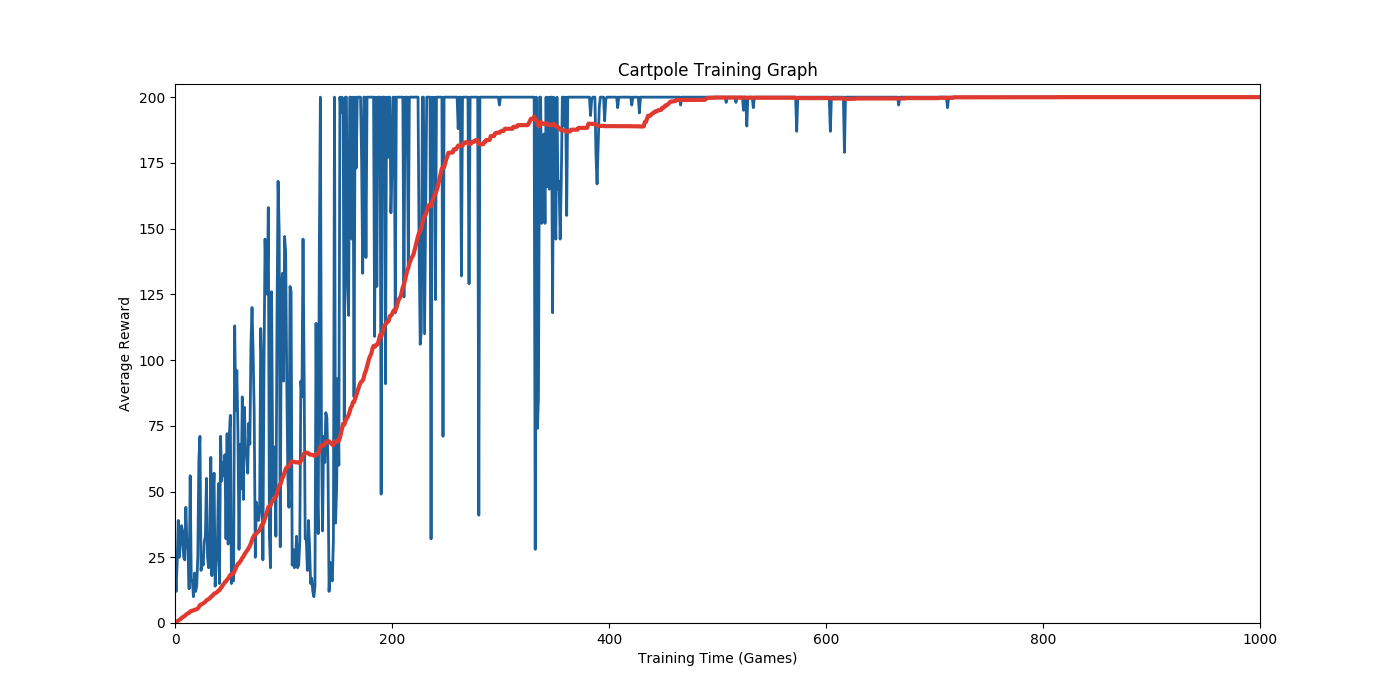
\includegraphics[scale=0.4]{images/Cartpole_Training_Graph.png}
            \caption{The average rewards achieved by the agent alongside it's training time}
            \label{fig:cartpole1}
        \end{figure}
        Figure \ref{fig:cartpole1} shows the training curve of Adam-DQL agent. The red line represents the average reward of the agent while the blue line represents the rolling mean of the agent's performance throughout the training process.
        \par
        One noticeable thing that stands out when we first see in Figure \ref{fig:cartpole1} is the
        oscillation of our agent's performance.This oscillation is due to our
        stochastic optimization procedure, Adam, considering different state-spaces within each step. It is obvious that this is not caused by an instability or diverging oscillations, simply because only the roling mean is oscillating, and not the average reward itself. The average reward itself keeps growing because despite the randomness of early training process, the neural network parameters is still updated towards the global minima, and allows for better policy overtime. Another form of proof for randomness is that the oscillation actually becomes smaller and smaller as the time goes on. This shows that the policy of the agent itself is becoming better, resulting in more consistent gameplay for the latter episodes. 
        
        \begin{figure}[H]
            \centering
            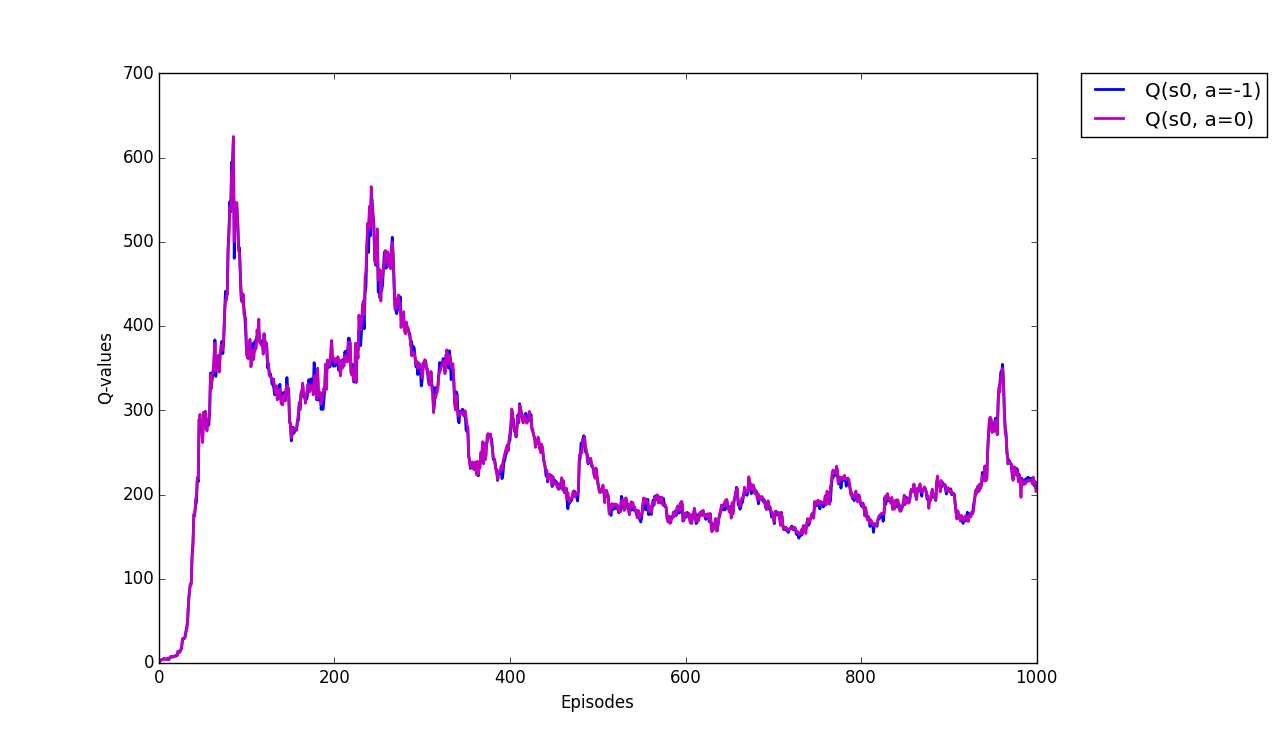
\includegraphics[scale=0.3]{images/qvaluecartpole.png}
            \caption{Q values at the start of every episode}
            \label{fig:cartpole2}
        \end{figure}
        Q-values from both actions are gathered and presented in Figure \ref{fig:cartpole2}. The starting state in each episode is not static. This is obvious because Cartpole problem spawns the cart on a random position, generating different starting dynamics each time. Nevertheless, our Q-network predicts an average of two hundred steps until failure, which is still above the "solved" flag consideration. The fact that these 2 graph almost coincide with each other shows how well Adam-DQL agent generalize or learn the game strategy. Because this 2 Q-values shows how consistent the agent performs despite being thrown on a slightly different starting condition. If the agent is overfitted on the training data, changing the starting condition will resulted in huge drop in agent performance.
        \iffalse
        \begin{figure}[H]
            \centering
            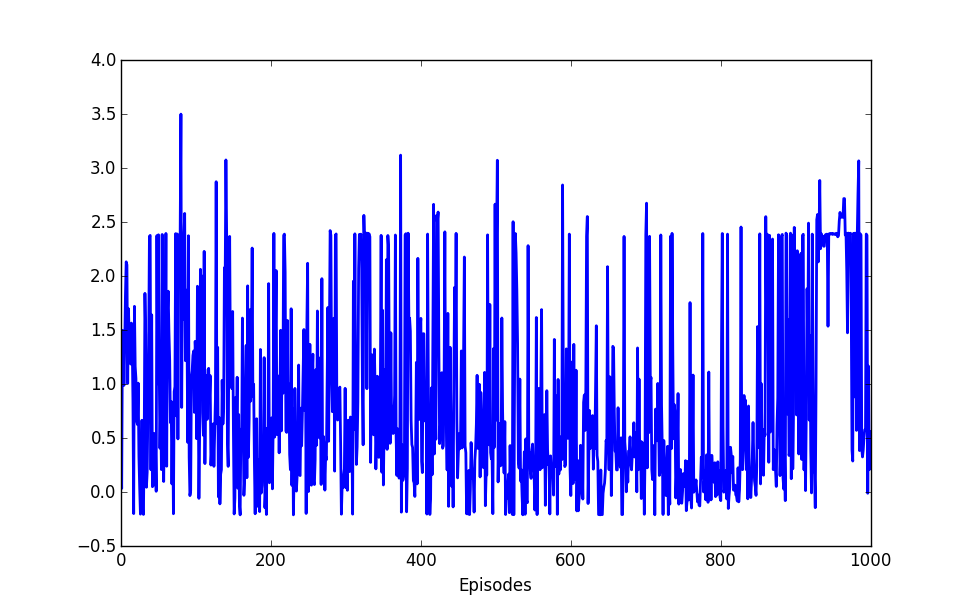
\includegraphics[scale=0.4]{images/value.png}
            \caption{Value function of the Cartpole problem}
            \label{fig:cartpole3}
        \end{figure}
        The value function varies from 0 to 2.5 (the correct value should be around 1). The oscillation is also due to the update-rate and the fact the optimization procedure derives from a stochastic sampling.
        \fi
        \par
         Despite showing steady improvements overtime, to further showcase both the capability and the practicality of Adam-DQL, it is needed to compare the results shown above with a previous work on the same environment. \cite{flappyDL} created an agent using Deep Q-Learning similar to Deepmind's \cite{mnih2015humanlevel} and trained the agent on the same CartPole environment:
         \begin{figure}[H]
             \centering
             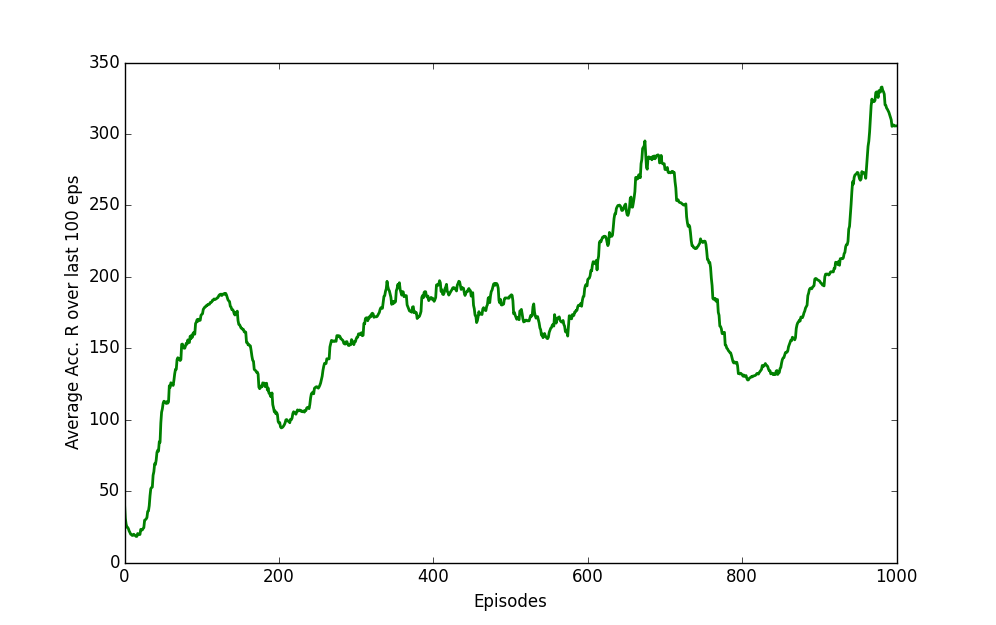
\includegraphics[scale=0.4]{images/rewardcartpole.png}
             \caption[Average Rewards for classiccal Deep Q-Learning Agent]{Average Rewards for classiccal Deep Q-Learning Agent \cite{lillicrap2015continuous}}
             \label{fig:cartpole4}
         \end{figure}
        
        It's clear that compared to Adam-DQL agent result shown in Figure \ref{fig:cartpole1}, classical Deep Q-Learning agent has much more noticeable stability issues on its learning curve. Classical Deep Q-Learning agent oscillates on the reward level, which means it actually has regression in its policy, that is not caused by the stochastic sampling. Adam-DQL agent only oscillates on the standard deviation level, which means that it still plays better overtime, but at the early stages, the quality of play is not as consistent as the later stages. However, classical Deep Q-Learning agent actually plays worse overtime on some intervals, which indicates that the policy itself its becoming worse. 
        \par
        This comes from the fact that Stochastic Gradient Descent (SGD) that is used in classical Deep Q-Learning doesn't account for the gradient historical data. This means, if at a time $t$ the computed gradient actually drives the current approximation away from global minima, the algorithm doesn't have any way to prevent the \textit{bad} gradient ruining the currently better policy. If this happens often, there might be a regression in policy, and thus the agent performance. In this case, it was clear that there's a regression around episode 200 and episode 400, where the agent performance goes downhill and doesn't go back up until few hundred episodes later.
         \par
        This thesis adds 2 additional policy improvement technique for deep Q-learning. However, none of this policy improvement technique will be applied on this problem. Partial training, the first policy improvement technique is inapplicable for this problem, because it is not possible to divide the cartpole problem into smaller subproblems that differs in difficulty. The second improvement, demonstration, is not necessary for this problem. Demonstration tries to help with the problem with a very sparse, hard to achieve reward. Because of how simple this problem is, random exploration is already more than enough to solve this game in a reasonable time. By observing Figure \ref{fig:cartpole1}, it is clear that this problem can be solved in way less than 1000 games. Which is considered instant by modern computing standards. Adding extra human-created transitions is overkill for this problem. 
         
    \subsection{FlapPy Bird}
        
    Our second task: FlapPy Bird is tested and further analyzed on our Adam-DQL agent. This environment is chosen to represent a set of problems where the playing strategy \textit{looks} simple, but it is hard pinpoint precisely, both from mathematical and programming standpoint. It might be possible to create a deterministic algorithm that \textit{somewhat solves} the problem. However it might be impossible to solve it completely. Our Adam-DQL agent is trained and tested on this problem, with the results shown below:
           \begin{figure}[H]
        \centering
        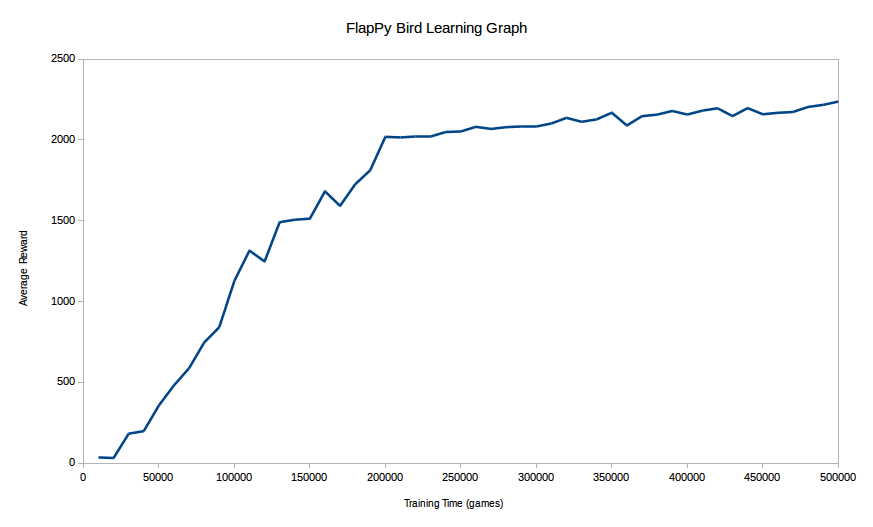
\includegraphics[scale=0.5]{images/flappyreward.png}
        \caption{The average rewards achieved by the agent alongside it's training time}
        \label{fig:flappy1}
    \end{figure}
    In this environment, instead of the global learning parameters $\epsilon=1$ annealed linearly until $\epsilon=0.1$, $\epsilon=0.01$ annealed until $\epsilon=0.001$ is chosen. This is inspired by \cite{flappyDL}. FlapPy Bird is a very fast environment, without a lot of slack time. This means if the agent decided to make a slight mistake, there's a high chance that the episode will end (the agent dies). If every time step, that is $\frac{1}{60}$ sec, $\epsilon=1$ until $0.1$, there's a very high chance that a random action is taken and since the environment only has 2 action, there's a very high chance that the agent will randomly \textit{flap}. If this happens often, which is very likely, the agent will die most of time hitting the pipe at the ceiling. For example, if $\epsilon=0.5$, there's a $\frac{1}{2} \times \frac{1}{2}$ chance that the bird will flap at every timestep. Which means the bird is expected to flap around 15 times in a second. This is way too frequent, and will simply result in the bird staying at the top of the screen. Hence, a really small $\epsilon$ is needed, thus the value $0,01$ annealed linearly to $0,001$ is selected.
    \par
    On this environment, understanding how our neural networks learn and knowing what information is considered \textbf{important} by our neural networks are vital. To achieve this, further analysis to our agents is performed. The output of our two convolutional neural networks is extracted and analyzed.
      \begin{figure}[H]
            \centering
            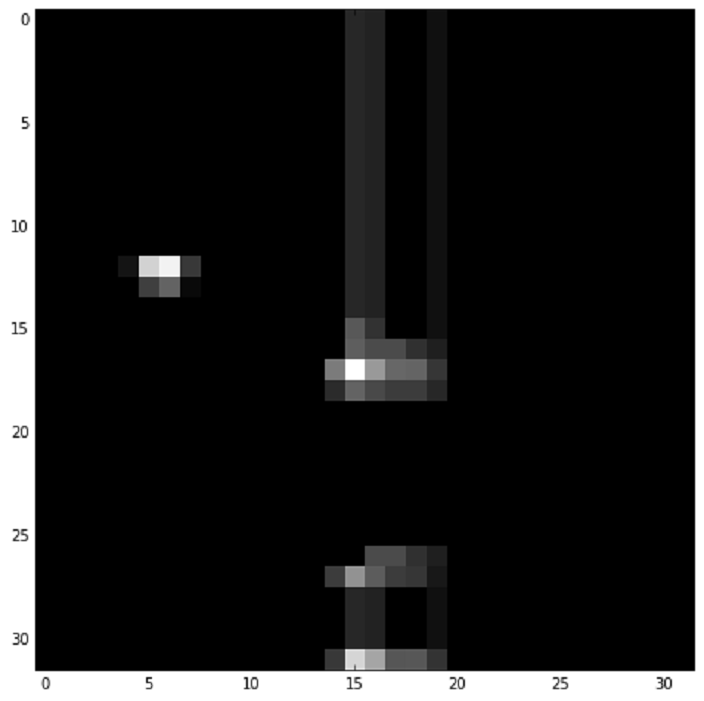
\includegraphics[scale=0.5]{images/layer1.png}
            \caption{The output of the first convolutional layers}
            \label{fig:flappy2}
        \end{figure}
    \begin{figure}[H]
            \centering
            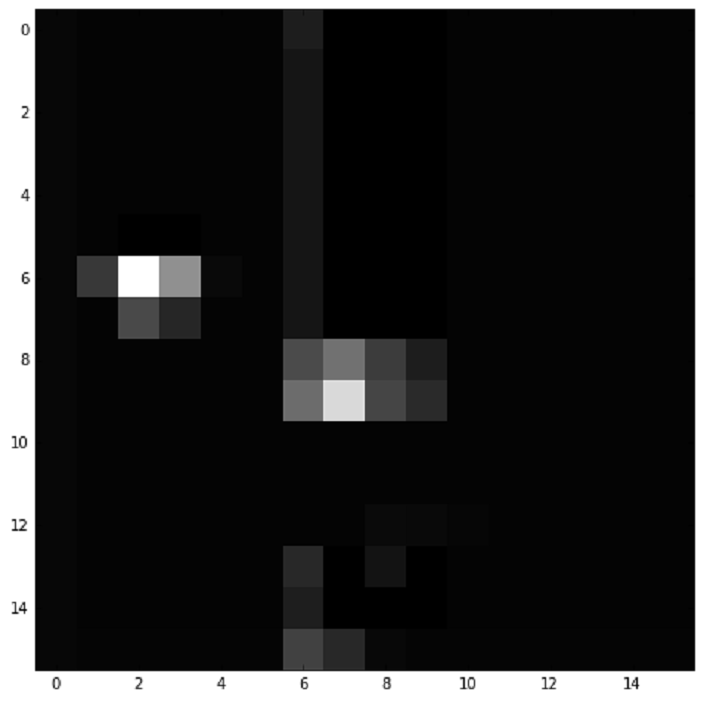
\includegraphics[scale=0.5]{images/layer2.png}
            \caption{The output of the second convolutional layers}
            \label{fig:flappy3}
        \end{figure}
    From Figure \ref{fig:flappy2} and \ref{fig:flappy3}, one can see that the \textbf{important} pixels are the position of the bird and gaps. Furthermore, seeing how the Figure \ref{fig:flappy2} is processed to become Figure \ref{fig:flappy3}, it is clear that the agent is trying to maintain the relative position between the bird and the gap. There's no scientific way to pinpoint how a convolutional neural network "\textit{learns}". However this two image outputs definitely gave some idea about how Adam-DQL agent can learn complex and advanced strategies about this game.
    \par
    Despite showing steady improvements overtime, to further showcase both the capability and the practicality of Adam-DQL, it is needed to compare the results shown above with a previous work on the same environment. \cite{flappyDL} created an agent using Deep Q-Learning similar to Deepmind's \cite{mnih2015humanlevel} and trained the agent on the same FlapPy Bird environment. The results of their work are shown alongside Adam-DQL's score in the table below:
    
        \begin{table}[H]
    \centering
        \label{flappycomparison}
    \begin{tabular}{|l|l|l|}
    \hline
    \# Training episodes     & Deep Q-Learning & Adam-DQL \\ \hline
    10000 (first checkpoint) & 11,6            & 35,1     \\ \hline
    99000                    & 1680,9          & 912,7   \\ \hline
    199000                   & 1026,8          & 1962,6   \\ \hline
    299000                   & 351,06          & 2058,1   \\ \hline
    399000                   & 1006,11         & 2179,4   \\ \hline
    \end{tabular}
    \caption[Average rewards of Adam-DQL FlapPy Bird agent compared to classical Deep Q-Learning agent]{Average rewards of Adam-DQL FlapPy Bird agent compared to classical Deep Q-Learning agent \cite{flappyDL} }
    \end{table}

    Not only that Adam-DQL agent performs better, it also doesn't suffer from regression through training overtime. Adam optimizer, the optimization algorithm for Adam-DQL is amplifying the gradient of the neural network using the first moment(means). This leads to neural network converging or reaching the global minima faster. Adam optimizer also prevents the instability (where the neural networks oscillate around a local minima) by scaling the gradients with second moment(uncentered variance). Because of these reasons, not only our Adam-DQL agent perform better with the same amount of training, it also doesn't suffer from regressions like what happened to the classical Deep Q-Learning that uses Stochastic Gradient Descent (SGD).
    
    As explained in Section \ref{sec:4}, Adam-DQL also implements a technique called \textbf{demonstration}. 100 sets of training data (transitions) are stored into the replay memory $D$ before the training start. This data is taken from human data playing the game for 100 frame sets. The demonstration data is by no means perfect, however this imperfect data will then be replaced by agent's replay memory. This idea is directly taken from \cite{DBLP:journals/corr/abs-1709-10089}, where the suboptimal demonstration data is handled in largely the same way.
    
       \begin{figure}[H]
        \centering
        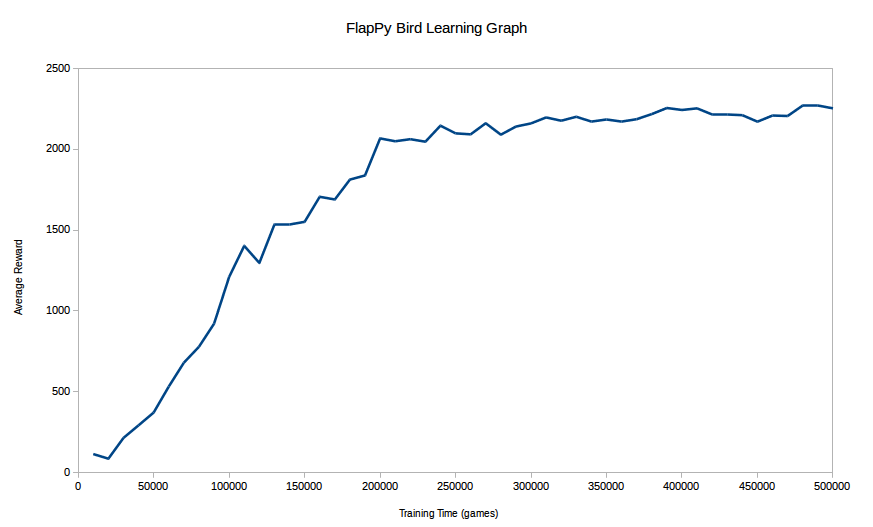
\includegraphics[scale=0.5]{images/flappyrewardemo.png}
        \caption{The reward graph for Adam-DQL with demonstration}
        \label{fig:flappy4}
    \end{figure}
    
    It is clear that there's a huge improvement in the first few training episodes. On the later stages of training process, the improvements over Adam-DQL without demonstration is very subtle. By giving initial "knowledge" to the agent, the agent can start improving pretty fast. Instead of random exploration in the start of the training process, the agent has a basic idea about how the game should be tackled, and explore from there. As explained before, this demonstrations data can be replaced by agent's memory later into the training process, which explain why the improvement on the later stage of the training process is very small. 
    \par
    There's also another improvement that can't be represented by a mere numbers. By kickstarting the agent's learning capability, there's a less chance that the agent will go into a feedback loop (where the agent can't improve because of bad training experience) or diverge catastrophically. Since deepmind proposed experience replay in \cite{mnih2015humanlevel}, there's only a small chance of this divergence actually happening. However, another improvement is certainly a good thing. A tabular comparison of Adam-DQL and Adam-DQL with demonstration is shown below:
    
      \begin{table}[H]
    \centering
        \label{flappycomparison2}
    \begin{tabular}{|l|l|l|}
    \hline
    \# Training episodes     &  Adam-DQL       & Adam-DQL-D \\ \hline
    10000 (first checkpoint) & 35,1            & 114,1     \\ \hline
    99000                    & 912,7           & 1026    \\ \hline
    199000                   & 1962,6          & 1838,7   \\ \hline
    299000                   & 2058,1          & 2141,6   \\ \hline
    399000                   & 2179,4          & 2257,7   \\ \hline
    \end{tabular}
    \caption[Average rewards of "naive" Adam-DQL and Adam-DQL with demonstrations] {Average rewards of "naive" Adam-DQL and Adam-DQL with demonstrations \cite{flappyDL} }
    \end{table}
    
    As with the cartpole problem, it is also not possible to apply partial training to this problem. Partial training requires a problem that can be broken down to subproblems, where each subproblems differ in difficulty. This game relies on putting pipes on different position, which clearly can't be broken down into subproblems, as a pipe with position $x$ isn't a subset of pipe with position $y$. Thus partial training won't be applied for this problem, despite the game being relatively hard.
    
    \subsection{Simplified Tetris}
    Our final task: simplified Tetris, is tested and analyzed on Adam-DQL. This environment is selected to represent a problem that is both hard to model, verify or even approximate \cite{DBLP:journals/corr/cs-CC-0210020}, which is why Tetris is considered NP-Complete. Not only it's hard to approximate a solution for Tetris, it's also hard to verify whether that solution is actually correct or not. For this reason, Tetris is considered an untouched problem in reinforcement learning, as it's hard to justify every actions and reward. Some researchers have attempted to solve Tetris as a reinforcement learning problem, albeit without a good results. This is why, this thesis is using a simplified version of tetris, instead of full version of Tetris with 6 type of tetrominis. This reduce the complexity of tetris to a reasonable degree. To further indicate how hard tetris is, below is the learning graph of "naive" Adam-DQL (without any policy improvement technique):
    
     \begin{figure}[H]
        \centering
        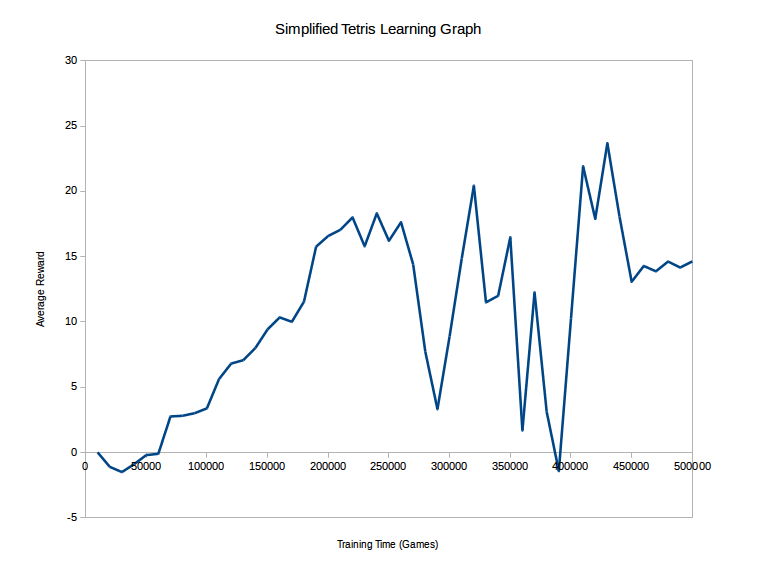
\includegraphics[scale=0.5]{images/tetrisreward.png}
        \caption{The average rewards achieved by the agent alongside it's training time}
        \label{fig:tetris1}
    \end{figure}
    
    It's really clear that the agent struggles to solve the problem. The reward graph oscillates extremely, indicating that there's no clear policy that the agent can infer from the environment. The reward at the end of the training is also way less than $100$, which indicates that the agent can't even clear $1$ line consistently for every game. Fortunately, there's a clear explanation about why this happened, and it has to do with the idea of Q-learning itself.
    \par
    From Chapter \ref{sec:4}, the bellman equation is defined as follows:
    \begin{equation*}
         Q_{i+1}(s,a)=\E[r+\gamma\max_{a'}Q_i^*(s',a')]
    \end{equation*} 
    Note that to update $Q(s,a)$, Q-learning relies on a term $r$, which is the reward term. To put it simply, if the agent doesn't get any reward in 2 subsequent states, $Q(s',a')=Q(s,a)$ and $r=0$, which means $Q(s,a)=0+Q(s',a')=Q(s,a)$. This also applies to deep Q-learning, where the neural network won't be able to learn unless it receives some rewards. At the start of the neural network, all the weights and parameters are initialized randomly, and $\epsilon$ is initialized to 1. This means before training, neural network is basically doing a random exploration. 
    \par
    Tetris is a different "type" of problem from FlapPy Bird and Cartpole. The later represents \textbf{reflex-based} games, where it relies on human reflexes combined with some strategy, while Tetris is a \text{strategy-based} game. This is really important, because on a game that relies on reflexes, using a random exploration might resulted in a reward. For a strategy game, an agent might need to do a set of planned strategy just to get a reward. By not getting any reward, the agent basically does a random exploration, but since the game needs a strategic planning, it will never get a reward, and so on. On robotic terms \cite{DBLP:journals/corr/abs-1709-10089}, problem like this is said to have \textbf{sparse} rewards.
    \par
    Deepmind's original deep Q-learning also struggles from the same problem \cite{mnih2015humanlevel}. While some games performed amazingly, game with sparse rewards struggles to even get a single reward. However, This doesn't mean that deep reinforcement learning in general is impossible for these kind of environments, as there's a possible solutions for this phenomenon. The main problem is that the agent can't get a reward, which means by giving some sort of help, the agent can start learning, and in the end, strategize for itself.
    \par 
    This is where our first policy improvement technique comes in, partial training, which is aimed to reduce the complexity and strategy needed to get a reward, is applied to our simplified Tetris environment. The environment is broken down into 2 subproblems, the first subproblem is a Tetris with only 1 tetrominis, the "O"(square) block. Randomly putting the square block into the grid has a reasonable chance clear a line, which means that the agent might receive a reward just by playing randomly. This subproblem is definitely easier to solve, and it helped our neural network to start learning. After trained to some extent, this agent is now much better prepared to solve the full environment with two blocks.
    
    
     \begin{figure}[H]
        \centering
        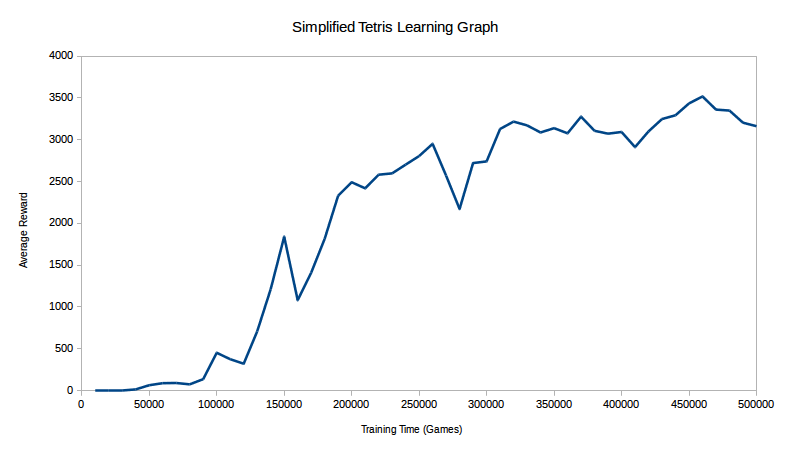
\includegraphics[scale=0.5]{images/tetrisreward2.png}
        \caption{TThe reward graph for Adam-DQL with partial training}
        \label{fig:tetris2}
    \end{figure}
    
    It is clear that from Figure \ref{fig:tetris2}, the difference made by implementing partial training is night and day. Not only the agent learn much more steadily (without extreme oscillation), the agent now can achieve around 3000-3500 reward points. This means our agent can clear on average 30 lines a game, which is a huge improvement from standard Adam-DQL.
    \par
    Demonstration, our second policy improvement technique is also applied and tested for Tetris environment. Demonstration tries to help the agent to get a reward with a different way. Instead of reducing the complexity of the problem, demonstration is aimed to give some initial strategy by feeding human-created transitions into agent memory. 100 frames of human-created transitions are stored into replay memory $D$ before the training process starts.
    
    \begin{figure}[H]
        \centering
        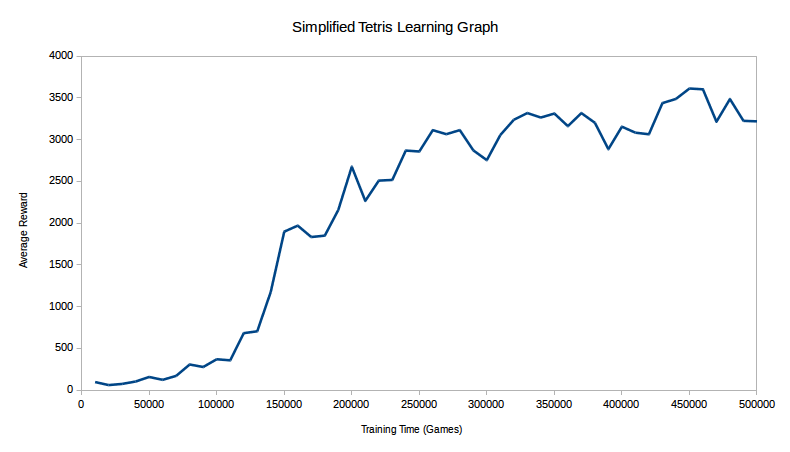
\includegraphics[scale=0.5]{images/tetrisreward3.png}
        \caption{The reward graph for Adam-DQL with partial training and demonstration}
        \label{fig:tetris3}
    \end{figure}    
    
    Clearly, from Figure \ref{fig:tetris3}, demonstration seems to help "lift" the early part of the training process. This synergizes with the idea that it tries to help initial training process. However, as with FlapPy Bird, demonstration doesn't seem to help with the later stages of training process. As it has almost identical reward as Figure \ref{fig:tetris3}. Again, this comes from the fact that the human-created transition is replaced after several training episodes.
    \par
    These 2 improvements on Adam-DQL dont simply make tetris completely solvable with Adam-DQL, however. On the later stages of training process, Figure \ref{fig:tetris2} and \ref{fig:tetris3} indicate that the performance of the agent got stuck around 3000 mark. From our extensive testing, this performance doesn't grow anymore with more training time. Which indicates there's something preventing the agent from learning more. From our analysis, this can be caused by 2 things:
    \begin{enumerate}
        \item The game has a really sparse rewards, which means that most of the time, the agent is gonna get 0 or even negative reward. Adam-DQN uses ReLU (rectified linear unit) which is defined as $\phi(x)= max(0,x)$. 
        Assume a very simple loss function $L(y)=\phi(\hat{y})-y$ is used, for a parameter $\theta_n$, there's only 2 possible gradient value:
        \begin{equation*}
            \frac{\partial L}{\partial \theta_n}=\delta_n=
            \begin{cases}
            1 & \theta_n \geq 0\\
            0 & \theta_n < 0
            \end{cases}
        \end{equation*}
        which simply means, if the value of a neuron is smaller than 0, the gradient will be 0 and the parameter won't be updated. Since  $\phi(0)$ is also 0, this will result in a dead neuron, which means this neuron won't be able to learn anything anymore.
        \item The reward for an action in Tetris is usually very delayed. Adam-DQL uses discounted future reward, which means a reward given on the 1000 timesteps ahead for example, is discounted by discount factor $\gamma^{100}$. This is a structural problem which is harder to solve, because the standard value for $\gamma$ is $0.99$, which is already really close to 1. Still, $0.99^{100}=0.366$, which is relatively small. This nullifies the value of that action to the final reward, making it harder for the agent to pinpoint which action produces a reward.
    \end{enumerate}
    
    This 2 problem is currently unsolved for Adam-DQL agent. However, this can be a guidance and idea for further research.
    
    